\documentclass[10pt,conference,letterpaper]{IEEEtran}
\providecommand{\DoNotLoadEpstopdf}{}
\usepackage[T1]{fontenc}
\usepackage{lmodern,amsmath,amssymb,graphicx,booktabs}
\usepackage{mathptmx}
\usepackage[scaled=.95]{helvet}
\usepackage[american]{circuitikz}
\usetikzlibrary{calc,positioning,arrows.meta,shapes.gates.logic.US}
% Shared by the report and every standalone PDF/SVG.
\ctikzset{
  transistors/scale=0.8,
  resistors/scale=0.5,
  capacitors/scale=0.5,
  sources/scale=0.8,
  logic ports/scale=0.6,
  flipflops/scale=0.6,
  tripoles/mos style=arrows,
  transistors/arrow pos=end,
  amplifiers/scale=0.7,
  blocks/scale=0.7
}
\newcommand{\ADCfigurefont}{\sffamily\bfseries}
\tikzset{every picture/.append style={line width=.60pt,
  font=\ADCfigurefont\footnotesize},
  adc block/.style={draw=black,fill=white,line width=.85pt,
    rounded corners=0pt,align=center,font=\ADCfigurefont\footnotesize},
  adc wire/.style={draw=black,line width=.60pt},
  adc group/.style={draw=none,fill=black!12},
  adc signal/.style={adc wire,-{Triangle[length=2.2mm,width=1.6mm]}},
  adc control/.style={adc signal,densely dashed},
  adc dot/.style={circle,fill=black,inner sep=1.15pt},
  adc net/.style={font=\ADCfigurefont\footnotesize,inner sep=1.5pt}}
\ctikzset{bipoles/thickness=1.25,tripoles/thickness=1.25}

\usepackage[hidelinks]{hyperref}
\hypersetup{pdftitle={An 8-bit 20-MS/s Differential SAR ADC},pdfauthor={SAR ADC Project},pdfsubject={Circuit implementation and historical schematic verification}}
\title{An 8-bit 20-MS/s Differential SAR ADC:\\Circuit Implementation and Schematic Verification}
\author{\IEEEauthorblockN{SAR ADC Project}\IEEEauthorblockA{Design and verification report}}
\begin{document}
\raggedbottom
\maketitle
\begin{abstract}
A differential charge-redistribution successive-approximation ADC combines an ideal binary capacitor array, a dynamic comparator with isolated static storage, and a transistor-level Johnson-counter controller. The schematic prototype operates at a nominal 20\,MS/s from a 0.9\,V supply. Two archived transient-noise records give 48.054 and 47.494\,dB SNDR at 1.328125 and 9.296875\,MHz. Five deterministic process-corner datasets observe all 256 output codes and bound endpoint-fit DNL and INL within the declared limits. A strict reverse-history comparison fails at the exact central transition and remains explicitly recorded. This report documents the implemented connections, historical results, and the limits of an ideal-capacitor, pre-layout prototype. Drawing and packaging the evidence do not constitute a new circuit simulation.
\end{abstract}
\begin{IEEEkeywords}
successive-approximation ADC, charge redistribution, dynamic comparator, transmission-gate storage, schematic verification
\end{IEEEkeywords}

\section{Design Objective and Evidence}
The implementation retains eight binary output decisions while adapting the conversion rate and supply to 20\,MS/s and 0.9\,V. A 200\,MHz external clock supplies ten slots per conversion: two nominal acquisition slots and eight comparisons. This operating point is a project target, not a maximum-speed claim. The nominal differential input range is 1\,V peak to peak with a 0.45\,V common mode. The ideal high and low references are 0.7 and 0.2\,V.

The repository contains authored connectivity and nominal device geometry, compact conversion-code exports, deterministic transition brackets, and analysis programs \cite{repo}. The circuit drawings in this report are derived from that connectivity. They are not an editable CAD database, a layout, or a claim that the symbolic model names reproduce the licensed transistor simulations.

\begin{table}[!b]\centering
\caption{Prototype operating point and retained evidence}\label{tab:overview}
\begin{tabular}{lr}\toprule
Quantity & Value\\\midrule
Nominal resolution & 8 bits / 256 codes\\
Sampling rate & 20\,MS/s\\
Supply / nominal temperature & 0.9\,V / 25\,$^\circ$C\\
Differential full scale & 1\,V peak to peak\\
Unit capacitor / each-side total & 5\,fF / 1.28\,pF\\
Expanded ADC MOS instances & 769\\
Noisy SNDR, low / high tone & 48.054 / 47.494\,dB\\
Noisy ENOB, low / high tone & 7.690 / 7.597\\
Worst static DNL magnitude bound & 0.251154\,LSB\\
Worst static INL magnitude bound & 0.190113\,LSB\\\bottomrule
\end{tabular}
\end{table}

\section{Differential Signal Path}
Fig.~\ref{fig:system} shows the top-level connection between the sampled capacitor-array top plates, comparator, and controller. The positive and negative arrays each contain eight binary-weighted branches and one dummy unit. With $C_u=5$\,fF,
\begin{equation}
C_{\mathrm{side}}=C_u\left(1+\sum_{k=0}^{7}2^k\right)=256C_u=1.28\,\mathrm{pF}.
\end{equation}
The dummy branch remains connected to common mode. During acquisition the input sampling gates connect the top plates to the differential input. Unresolved conversion branches connect their bottom plates to common mode. Resolved branches switch to complementary reference levels. A positive comparison selects the differential subtracting DAC step.

\begin{figure*}[!t]\centering
\resizebox{.96\textwidth}{!}{\begin{circuitikz}[x=1cm,y=1cm]
\node[adc block,minimum width=3.2cm,minimum height=2.2cm] (dac) at (3.4,3.8)
  {Differential CDAC\\$C_u=5\,\mathrm{fF}$\\$256C_u$ per side};
\node[adc block,minimum width=3.1cm,minimum height=2.2cm] (cmp) at (8.1,3.8)
  {Dynamic comparator\\isolation buffers\\NAND SR hold};
\path[adc group] (1.5,-.5) rectangle (13.8,1.9);
\node[adc block,minimum width=4.7cm,minimum height=1.25cm] (seq) at (4.3,.6)
  {5-stage Johnson counter\\interlocked phases / bit latches};
\node[adc block,minimum width=3.2cm,minimum height=1.25cm] (out) at (10.7,.6)
  {8 output latches\\$D_7\ldots D_0$};
\node[adc net,anchor=west] at (8.6,-.3) {Native SAR controller};
\draw[adc signal] (0,4.35) node[left] {$V_{\!IP}$} -- (1.8,4.35);
\draw[adc signal] (0,3.25) node[left] {$V_{\!IN}$} -- (1.8,3.25);
\draw[adc signal] (5,4.35) -- (6.55,4.35) node[midway,above] {$v_p$};
\draw[adc signal] (5,3.25) -- (6.55,3.25) node[midway,above] {$v_n$};
\draw[adc signal] (9.65,3.8) -- (12.8,3.8) node[midway,above] {$\mathrm{cmpQ}$}
  -- (12.8,2.2) -- (5.2,2.2) -- (5.2,1.225);
\draw[adc control] (2.4,1.225) -- (2.4,2.7) node[midway,left] {track};
\draw[adc control] (3.4,1.225) -- (3.4,2.7) node[midway,right] {$b_{7:0},v_{7:0}$};
\draw[adc control] (6.65,.6) -- (7.3,.6) -- (7.3,2.7) node[midway,left] {cmpclk};
\draw[adc signal] (6.65,.25) -- (9.1,.25) node[midway,below] {$b_{7:0}$};
\draw[adc control] (6.65,.95) -- (9.1,.95) node[pos=.65,above,align=center] {output\\enable};
\draw[adc signal] (12.3,.6) -- (14.5,.6) node[right,align=left] {8-bit\\output};
\draw[adc control] (0,.6) node[left,align=center] {200 MHz\\CLK} -- (1.95,.6);
\draw (0,-1) node[vcc] {$V_{\!DD}$} to[C,l=$1\,\mathrm{pF}$] (0,-2.4)
  node[circ] {} to[R,l_=$100\,\mathrm{k}\Omega$] (0,-4) node[ground] {};
\node[not port] (pi0) at (1.7,-2.4) {};
\node[not port] (pi1) at (3.1,-2.4) {};
\draw (0,-2.4) -- (pi0.in) node[midway,above] {por};
\draw (pi0.out) -- (pi1.in) node[midway,above] {porb};
\draw[adc control] (pi1.out) -- (4.3,-2.4) -- (4.3,-.025)
  node[pos=.55,right] {RST};
\node[adc net,anchor=west,align=left] at (5.7,-2.25)
  {Internal power-on reset\\requires an actual supply ramp};
\draw[adc signal] (3.4,6) node[above,align=center] {$V_{\!REFP}=0.7$ V, $V_{\!REFN}=0.2$ V\\$V_{\!CM}=0.45$ V} -- (3.4,4.9);
\node[adc net,anchor=west] at (8.2,5.65) {$V_{\!DD}=0.9$ V; $f_s=20$ MS/s};
\node[adc net,anchor=west] at (8.2,5.15) {2 acquisition + 8 comparison slots};
\end{circuitikz}
}
\caption{Implemented ADC hierarchy. Solid arrows carry analog signals or comparison data; dashed arrows carry switching and clock controls. The analog array and comparator are closed by the native controller. Ideal external references and the external clock are testbench boundaries. The shaded region groups the controller; it does not imply a separate power domain.}\label{fig:system}
\end{figure*}

Fig.~\ref{fig:cdac} retains both complete binary arrays rather than replacing their weights with an unspecified DAC block. The least-significant capacitor is physically present. The last comparison supplies the least-significant decision without a following LSB DAC update: the controller holds the corresponding valid flag low.

\begin{figure*}[!t]\centering
\resizebox{.95\textwidth}{!}{% @passive sar_cdac CDUMMYp capacitor vp vcm c=5e-15
% @passive sar_cdac CDUMMYn capacitor vn vcm c=5e-15
% @passive sar_cdac Cp7 capacitor vp botp7 c=6.4e-13
% @passive sar_cdac Cn7 capacitor vn botn7 c=6.4e-13
% @passive sar_cdac Cp6 capacitor vp botp6 c=3.2e-13
% @passive sar_cdac Cn6 capacitor vn botn6 c=3.2e-13
% @passive sar_cdac Cp5 capacitor vp botp5 c=1.6e-13
% @passive sar_cdac Cn5 capacitor vn botn5 c=1.6e-13
% @passive sar_cdac Cp4 capacitor vp botp4 c=8e-14
% @passive sar_cdac Cn4 capacitor vn botn4 c=8e-14
% @passive sar_cdac Cp3 capacitor vp botp3 c=4e-14
% @passive sar_cdac Cn3 capacitor vn botn3 c=4e-14
% @passive sar_cdac Cp2 capacitor vp botp2 c=2e-14
% @passive sar_cdac Cn2 capacitor vn botn2 c=2e-14
% @passive sar_cdac Cp1 capacitor vp botp1 c=1e-14
% @passive sar_cdac Cn1 capacitor vn botn1 c=1e-14
% @passive sar_cdac Cp0 capacitor vp botp0 c=5e-15
% @passive sar_cdac Cn0 capacitor vn botn0 c=5e-15
% Source: sar_cdac. The two arrays are identical except bottom-plate polarity.
% All nine capacitors per side shown; ideal values, no physical cap geometry.
\begin{circuitikz}
\foreach \side/\yy/\nodev in {p/5.4/v_p,n/1.7/v_n}{
 \draw (1,\yy)--(15.2,\yy);
 \node[left] at (1,\yy) {$\nodev$};
 \foreach \bit/\xx/\val in {7/2/128,6/3.45/64,5/4.9/32,4/6.35/16,3/7.8/8,2/9.25/4,1/10.7/2,0/12.15/1}{
  \draw (\xx,\yy) node[adc dot] {} to[C,l_={$\val C_u$}] (\xx,\yy-1.4)
    -- (\xx,\yy-1.7) node[below] {$bot_{\side\bit}$};
 }
 \draw (14.1,\yy) node[adc dot] {} to[C,l_={$C_u$}] (14.1,\yy-1.4)
 --(14.1,\yy-1.7) node[below] {$V_{\mathrm{CM}}$};
}
\node[above] at (8.2,5.8) {$C_u=5\,\mathrm{fF},\qquad C_{\mathrm{side}}=256C_u=1.28\,\mathrm{pF}$};
\node[align=left,anchor=west] at (1,-1.3) {Each $bot_{pi}$ and $bot_{ni}$ connects to its three-way TG selector.\\Sampling: two parallel NMOS and two parallel PMOS per input side.};
\end{circuitikz}
}
\caption{Differential binary CDAC. Each side has weights $128{:}64{:}32{:}16{:}8{:}4{:}2{:}1$ plus one common-mode dummy. Each labeled bottom-plate net connects to the corresponding selector in Fig.~\ref{fig:cdacswitch}. All capacitors are ideal schematic elements; the drawing assigns no physical capacitor dimensions or mismatch.}\label{fig:cdac}
\end{figure*}

\subsection{Sampling and Bottom-Plate Selection}
The sampling gate on each input contains two explicit parallel NMOS/PMOS pairs. Each individual device has a nominal width of 3\,$\mu$m and length of 30\,nm. Thus each sampling polarity has a total nominal parallel width of 6\,$\mu$m. Each bottom-plate selection path instead contains one 3\,$\mu$m NMOS/PMOS pair. Separate explicit instances are not interchangeable with an unspecified multiplicity or finger parameter.

The selector controls satisfy $e_k=v_k\overline{\mathrm{track}}$, $h_k=e_kb_k$, and $l_k=e_k\overline b_k$. The common-mode path is enabled by $\overline e_k$. When $h_k$ is active, the positive-side bottom plate connects to the low reference and the negative-side bottom plate to the high reference. When $l_k$ is active, those assignments reverse. This polarity is part of the implemented SAR feedback, not a cosmetic labeling choice.

\begin{figure*}[!t]\centering
\resizebox{.95\textwidth}{!}{% @mos sar_cdac MSNp0 NMOS vp track vip vss 3e-06 3e-08
% @mos sar_cdac MSPp0 PMOS vp trackb vip vdd 3e-06 3e-08
% @mos sar_cdac MSNp1 NMOS vp track vip vss 3e-06 3e-08
% @mos sar_cdac MSPp1 PMOS vp trackb vip vdd 3e-06 3e-08
% @mos sar_cdac MSNn0 NMOS vn track vin vss 3e-06 3e-08
% @mos sar_cdac MSPn0 PMOS vn trackb vin vdd 3e-06 3e-08
% @mos sar_cdac MSNn1 NMOS vn track vin vss 3e-06 3e-08
% @mos sar_cdac MSPn1 PMOS vn trackb vin vdd 3e-06 3e-08
% @mos sar_cdac MNHp7 NMOS botp7 hi7 refn vss 3e-06 3e-08
% @mos sar_cdac MPHp7 PMOS botp7 hib7 refn vdd 3e-06 3e-08
% @mos sar_cdac MNLp7 NMOS botp7 lo7 refp vss 3e-06 3e-08
% @mos sar_cdac MPLp7 PMOS botp7 lob7 refp vdd 3e-06 3e-08
% @mos sar_cdac MNMp7 NMOS botp7 eb7 vcm vss 3e-06 3e-08
% @mos sar_cdac MPMp7 PMOS botp7 e7 vcm vdd 3e-06 3e-08
% @mos sar_cdac MNHn7 NMOS botn7 hi7 refp vss 3e-06 3e-08
% @mos sar_cdac MPHn7 PMOS botn7 hib7 refp vdd 3e-06 3e-08
% @mos sar_cdac MNLn7 NMOS botn7 lo7 refn vss 3e-06 3e-08
% @mos sar_cdac MPLn7 PMOS botn7 lob7 refn vdd 3e-06 3e-08
% @mos sar_cdac MNMn7 NMOS botn7 eb7 vcm vss 3e-06 3e-08
% @mos sar_cdac MPMn7 PMOS botn7 e7 vcm vdd 3e-06 3e-08
% Source-derived representative positive-side bit i and sampling pair.
% D/G/S/B of each representative switch is stated in the report's mapping table.
\begin{circuitikz}
% Actual parallel MOS topology of sampling: show one pair, explicit x2.
\node[nmos,rotate=-90] (sn) at (2,4.3) {};
\node[pmos,rotate=90] (sp) at (2,2.7) {};
\draw (sn.S)--(.9,4.3)--(.9,2.7)--(sp.S);
\draw (sn.D)--(3.1,4.3)--(3.1,2.7)--(sp.D);
\draw (.9,3.5) node[adc dot] {}--(.1,3.5) node[left] {$VIP$};
\draw (3.1,3.5) node[adc dot] {}--(3.9,3.5) node[right] {$v_p$};
\draw (sn.G)--++(0,.25) node[above] {$track$};
\draw (sp.G)--++(0,-.25) node[below] {$\overline{track}$};
\node[above] at (2,6.1) {Sampling pair ($\times 2$)};
\node[align=center] at (2,.3) {$W_n=W_p=3\,\mu\mathrm{m}$\\$L_n=L_p=30\,\mathrm{nm}$};
% Three explicit CMOS transmission gates, shared drain node.
\foreach \yy/\nn/\en/\eb/\src in {6.5/H/hi_i/\overline{hi_i}/V_{\mathrm{REFN}},3.5/L/lo_i/\overline{lo_i}/V_{\mathrm{REFP}},.5/M/\overline{e_i}/e_i/V_{\mathrm{CM}}}{
 \node[nmos,rotate=-90] (n\nn) at (8.6,\yy+.4) {};
 \node[pmos,rotate=90] (p\nn) at (8.6,\yy-.4) {};
 \draw (n\nn.S)--(7.6,\yy+.4)--(7.6,\yy-.4)--(p\nn.S);
 \draw (n\nn.D)--(9.6,\yy+.4)--(9.6,\yy-.4)--(p\nn.D);
 \draw (7.6,\yy) node[adc dot] {}--(6.5,\yy) node[left] {$\src$};
 \draw (9.6,\yy) node[adc dot] {}--(11,\yy);
 \draw (n\nn.G)--++(0,.12) node[right,inner sep=2pt] {$\en$};
 \draw (p\nn.G)--++(0,-.16) node[left,inner sep=2pt] {$\eb$};
}
\draw (11,.5)--(11,6.5);
\draw (11,3.5) node[adc dot] {} to[C,l={$2^i C_u$}] (13.1,3.5)--(13.6,3.5) node[right] {$v_p$};
\node[above right] at (11,3.5) {$bot_{pi}$};
\node[align=left,anchor=west] at (11,.65) {$e_i=v_i\,\overline{track}$\\$hi_i=e_i b_i$\\$lo_i=e_i\overline{b_i}$};
\node[align=center] at (8.4,-1.5) {Bottom-plate TGs: $W_n=W_p=3\,\mu\mathrm{m}$; $L=30\,\mathrm{nm}$.};
\node[align=center] at (7,-2.4) {NMOS bulks: $V_{\mathrm{SS}}$; PMOS bulks: $V_{\mathrm{DD}}$.\\Negative side: $VIP\to VIN$, $v_p\to v_n$, $V_{\mathrm{REFP}}\leftrightarrow V_{\mathrm{REFN}}$.};
\end{circuitikz}
}
\caption{Sampling and reference-selection circuits derived from the transistor connectivity. The sampler uses two parallel pairs per input; each selector uses one pair per reference/common-mode path. NMOS bulks connect to the negative supply and PMOS bulks to the positive supply. Equal labels identify connected nets. The negative-side selector uses the same controls with the high/low reference assignments exchanged.}\label{fig:cdacswitch}
\end{figure*}

\section{Comparator and Decision Storage}
The dynamic comparator contains an input differential pair, a clocked tail, a cross-coupled regenerative stage, and four PMOS reset devices. Four inverters isolate the regenerative nodes from a cross-coupled NAND storage pair (Fig.~\ref{fig:comparator}). The held decision remains available while the dynamic stage resets.

The comparator contains 11 direct MOS instances, eight MOS in the four inverters, and eight MOS in the two NAND gates, for 27 expanded instances. Device labels and internal nodes follow the source. The small-signal, reset, and regeneration behavior depends on the complete authorized device cards; nominal width and length alone do not recreate those cards.

\begin{figure*}[!t]\centering
\resizebox{.96\textwidth}{!}{% Source: design/adc_topology.scs, sar_comparator.
% @mos sar_comparator M1 NMOS p ip tail vss 3e-6 30e-9
% @mos sar_comparator M2 NMOS n in tail vss 3e-6 30e-9
% @mos sar_comparator M3 NMOS x y p vss 1e-6 30e-9
% @mos sar_comparator M4 NMOS y x n vss 1e-6 30e-9
% @mos sar_comparator M5 PMOS x y vdd vdd 1e-6 30e-9
% @mos sar_comparator M6 PMOS y x vdd vdd 1e-6 30e-9
% @mos sar_comparator M7 NMOS tail clk vss vss 3e-6 30e-9
% @mos sar_comparator MPp PMOS p clk vdd vdd 1e-6 30e-9
% @mos sar_comparator MPn PMOS n clk vdd vdd 1e-6 30e-9
% @mos sar_comparator MPx PMOS x clk vdd vdd 1e-6 30e-9
% @mos sar_comparator MPy PMOS y clk vdd vdd 1e-6 30e-9
% @instance sar_comparator XBX0 sar_inv vdd vss x xb
% @instance sar_comparator XBX1 sar_inv vdd vss xb xd
% @instance sar_comparator XBY0 sar_inv vdd vss y yb
% @instance sar_comparator XBY1 sar_inv vdd vss yb yd
% @instance sar_comparator XLQ sar_nand2 vdd vss xd qb q
% @instance sar_comparator XLQB sar_nand2 vdd vss yd q qb
\begin{circuitikz}
\node[nmos] (m1) at (1,1.5) {};
\node[nmos,xscale=-1] (m2) at (5,1.5) {};
\node[nmos] (m3) at (1,3.25) {};
\node[nmos,xscale=-1] (m4) at (5,3.25) {};
\node[pmos] (m5) at (1,5) {};
\node[pmos,xscale=-1] (m6) at (5,5) {};
\node[nmos] (m7) at (3,-.1) {};
\draw (m5.S) -- (1,5.9) -- (5,5.9) -- (m6.S);
\node[above] at (3,5.9) {$V_{\mathrm{DD}}$};
\draw (m5.D) -- (m3.D) (m6.D) -- (m4.D);
\draw (m3.S) -- (m1.D) (m4.S) -- (m2.D);
\draw (m1.S) -- (1,.65) -- (5,.65) -- (m2.S);
\draw (3,.65) node[adc dot] {} -- (m7.D);
\draw (m7.S) -- (3,-1) node[ground] {};
\draw (m1.G) -- ++(-.45,0) node[left] {$v_p\;(ip)$};
\draw (m2.G) -- ++(.45,0) node[right] {$v_n\;(in)$};
\draw (m7.G) -- ++(-.45,0) node[left] {$\phi_c\;(clk)$};
\foreach \i/\gate in {3/y,5/y}{\draw (m\i.G) -- ++(-.35,0) node[left] {$\gate$};}
\foreach \i/\gate in {4/x,6/x}{\draw (m\i.G) -- ++(.35,0) node[right] {$\gate$};}
\draw (1,4.12) node[adc dot] {} -- ++(-.6,0) node[left] {$x$};
\draw (5,4.12) node[adc dot] {} -- ++(.6,0) node[right] {$y$};
\draw (1,2.35) node[adc dot] {} -- ++(-.6,0) node[left] {$p$};
\draw (5,2.35) node[adc dot] {} -- ++(.6,0) node[right] {$n$};
\node[above] at (3,.65) {$tail$};
\foreach \i in {1,3,5}{\node[right] at (m\i.D) {$M_{\i}$};}
\foreach \i in {2,4,6}{\node[left] at (m\i.D) {$M_{\i}$};}
\node[right] at (m7.D) {$M_7$};
\node at (3,-1.65) {(a) Regenerative core};
% Four reset PMOS devices are shown separately, with connected net labels.
\foreach \xx/\nn in {8.5/p,10.6/n,12.7/x,14.8/y}{
 \node[pmos] (r\nn) at (\xx,5) {};
 \draw (r\nn.S) -- (\xx,5.9);
 \draw (r\nn.D) -- (\xx,4.15) node[below] {$\nn$};
 \draw (r\nn.G) -- ++(-.2,0) node[left] {$\phi_c$};
 \node[right] at (r\nn.D) {$M_{P\nn}$};
}
\draw (8.5,5.9)--(14.8,5.9);
\node[above] at (11.65,5.9) {$V_{\mathrm{DD}}$};
\node at (11.65,3.65) {(b) Precharge: $\phi_c=0$};
% Two CMOS inverters per path; cross-coupled NAND SR hold.
\node[not port] (bx0) at (8.5,2.35) {};
\node[not port] (bx1) at (10.4,2.35) {};
\node[not port] (by0) at (8.5,.35) {};
\node[not port] (by1) at (10.4,.35) {};
\node[nand port] (lq) at (13.6,2.35) {};
\node[nand port] (lqb) at (13.6,.35) {};
\draw (bx0.in)--++(-.35,0) node[left] {$x$};
\draw (by0.in)--++(-.35,0) node[left] {$y$};
\draw (bx0.out)--node[above] {$x_b$}(bx1.in);
\draw (by0.out)--node[above] {$y_b$}(by1.in);
\draw (bx1.out)--(11.7,2.35)|-node[pos=.25,above] {$x_d$}(lq.in 1);
\draw (by1.out)--(11.7,.35)|-node[pos=.25,above] {$y_d$}(lqb.in 1);
\draw (lq.in 2)--++(-.5,0) node[left] {$q_b$};
\draw (lqb.in 2)--++(-.5,0) node[left] {$q$};
\draw[adc signal] (lq.out)--++(.8,0) node[right] {$q$};
\draw[adc signal] (lqb.out)--++(.8,0) node[right] {$q_b$};
\node at (11.5,-.4) {(c) Isolation buffers and SR hold};
\node[align=center] at (11.5,-1.35) {All NMOS bulks: $V_{\mathrm{SS}}$; all PMOS bulks: $V_{\mathrm{DD}}$.\\Equal net labels denote electrical connections.};
\end{circuitikz}
}
\caption{Dynamic comparator, isolation inverters, and NAND SR hold. The cross-coupled gate connections and reset connections follow the published netlist. All dimensions in Table~\ref{tab:compgeom} are nominal requested geometry. Equal named nodes are connected even when a long return wire is omitted for clarity.}\label{fig:comparator}
\end{figure*}

\begin{table}[!t]\centering
\caption{Comparator nominal geometry; all $L=30$\,nm}\label{tab:compgeom}
\begin{tabular}{llr}\toprule
Devices & Type & Unit $W$ ($\mu$m)\\\midrule
$M_1,M_2,M_7$ & NMOS & 3\\
$M_3,M_4$ & NMOS & 1\\
$M_5,M_6$ & PMOS & 1\\
$M_{Pp},M_{Pn},M_{Px},M_{Py}$ & PMOS & 1\\
Each isolation inverter & NMOS / PMOS & 0.5 / 1\\
Each NAND device & NMOS / PMOS & 1 / 1\\\bottomrule
\end{tabular}
\end{table}

\section{Static Storage and Conversion Sequencing}
The controller uses the CMOS cells in Fig.~\ref{fig:logic-cells}, not ideal
logic sources. Figure~\ref{fig:logic-latch} expands its resettable storage
hierarchy. With $en=1$, the input transmission gate conducts and the feedback
gate opens. With $en=0$, the feedback gate retains the state. Pulling
$nrst=\overline{RST}$ low forces the NAND output $qb$ high and the final
output $q$ low. The formal $rst$ latch port is retained in the hierarchy;
the reset-to-zero action is applied through $nrst$.

\begin{figure*}[!t]
\centering
\resizebox{.97\textwidth}{!}{% Direct terminal order is D G S B; dimensions are nominal W L in metres.
% @mos sar_inv Mp PMOS y a vdd vdd 1e-6 30e-9
% @mos sar_inv Mn NMOS y a vss vss .5e-6 30e-9
% @mos sar_nand2 Mp0 PMOS y a vdd vdd 1e-6 30e-9
% @mos sar_nand2 Mp1 PMOS y b vdd vdd 1e-6 30e-9
% @mos sar_nand2 Mn0 NMOS y a ns vss 1e-6 30e-9
% @mos sar_nand2 Mn1 NMOS ns b vss vss 1e-6 30e-9
% @mos sar_tg Mn NMOS y en a vss .5e-6 30e-9
% @mos sar_tg Mp PMOS y enb a vdd 1e-6 30e-9
\begin{circuitikz}
% (a) CMOS inverter; named terminals follow the exported device order.
\node[pmos] (ip) at (1.65,4.0) {};
\node[nmos] (in) at (1.65,1.65) {};
\draw (ip.S) -- (1.65,5.05) node[above] {$V_{\mathrm{DD}}$};
\draw (in.S) -- (1.65,.70) node[ground] {};
\draw (ip.D) -- (in.D);
\draw (ip.G) -- (.35,4.0) -- (.35,1.65) -- (in.G);
\draw (.35,2.8) node[adc dot] {} -- (-.2,2.8) node[left] {$a$};
\draw (1.65,2.8) node[adc dot] {} -- (2.7,2.8) node[right] {$y$};
\node[right] at (ip.D) {$M_p$};
\node[right] at (in.D) {$M_n$};
\node[align=center] at (1.4,-1.0) {(a) Inverter\\$W_p/W_n=1/0.5\;\mu\mathrm{m}$};
% (b) NAND2: parallel PMOS pull-up and series NMOS pull-down.
\node[pmos] (np0) at (5.4,4.0) {};
\node[pmos,xscale=-1] (np1) at (7.8,4.0) {};
\node[nmos] (nn0) at (6.6,2.15) {};
\node[nmos] (nn1) at (6.6,.65) {};
\draw (np0.S) -- (5.4,5.05) -- (7.8,5.05) -- (np1.S);
\node[above] at (6.6,5.05) {$V_{\mathrm{DD}}$};
\draw (np0.D) -- (5.4,3.1) -- (7.8,3.1) -- (np1.D);
\draw (6.6,3.1) node[adc dot] {} -- (nn0.D);
\draw (7.8,3.1) node[adc dot] {} -- (8.55,3.1) node[right] {$y$};
\draw (nn0.S) -- (nn1.D);
\draw (6.6,1.38) node[adc dot] {} -- (7.15,1.38) node[right] {$ns$};
\draw (nn1.S) -- (6.6,-.15) node[ground] {};
\draw (np0.G) -- ++(-.35,0) node[left] {$a$};
\draw (np1.G) -- ++(.35,0) node[right] {$b$};
\draw (nn0.G) -- ++(-.35,0) node[left] {$a$};
\draw (nn1.G) -- ++(-.35,0) node[left] {$b$};
\node[right] at (np0.D) {$M_{p0}$};
\node[left] at (np1.D) {$M_{p1}$};
\node[right] at (7.0,2.15) {$M_{n0}$};
\node[right] at (7.0,.65) {$M_{n1}$};
\node[align=center] at (6.6,-1.0) {(b) NAND2\\All four widths: $1\;\mu\mathrm{m}$};
% (c) Parallel complementary pass devices; a is the declared source.
\node[nmos,rotate=-90] (tn) at (12.35,3.65) {};
\node[pmos,rotate=90] (tp) at (12.35,1.95) {};
\draw (tn.S) -- (11.2,3.65) -- (11.2,1.95) -- (tp.S);
\draw (tn.D) -- (13.5,3.65) -- (13.5,1.95) -- (tp.D);
\draw (11.2,2.8) node[adc dot] {} -- (10.6,2.8) node[left] {$a$};
\draw (13.5,2.8) node[adc dot] {} -- (14.1,2.8) node[right] {$y$};
\draw (tn.G) -- ++(0,.4) node[above] {$en$};
\draw (tp.G) -- ++(0,-.4) node[below] {$enb$};
\node[above left] at (tn.S) {$M_n$};
\node[below left] at (tp.S) {$M_p$};
\node[align=center] at (12.35,-1.0) {(c) Transmission gate\\$W_n/W_p=0.5/1\;\mu\mathrm{m}$};
\node[align=center] at (7.0,-2.0) {All $L=30\;\mathrm{nm}$. NMOS bulk: $V_{\mathrm{SS}}$; PMOS bulk: $V_{\mathrm{DD}}$.\\Equal labels denote the same net; dots mark junctions. Ground denotes $V_{\mathrm{SS}}$.};
\end{circuitikz}
}
\caption{Source-derived transistor implementations of the standard inverter,
NAND2 and transmission gate. Each cell uses its own local net names. NMOS
bulks connect to $V_{\mathrm{SS}}$ and PMOS bulks to $V_{\mathrm{DD}}$;
the three-terminal symbols omit these common body wires. Dimensions are
nominal requested geometry, not extracted dimensions or a replacement model card.}
\label{fig:logic-cells}
\end{figure*}

\begin{table}[!t]\centering
\caption{Logic-device terminal order $(D,G,S,B)$}
\label{tab:logic-terminals}
\begin{tabular}{lll}\toprule
Cell & Device & $(D,G,S,B)$\\\midrule
Inverter & $M_p$ & $(y,a,vdd,vdd)$\\
 & $M_n$ & $(y,a,vss,vss)$\\
NAND2 & $M_{p0}$ & $(y,a,vdd,vdd)$\\
 & $M_{p1}$ & $(y,b,vdd,vdd)$\\
 & $M_{n0}$ & $(y,a,ns,vss)$\\
 & $M_{n1}$ & $(ns,b,vss,vss)$\\
TG & $M_n$ & $(y,en,a,vss)$\\
 & $M_p$ & $(y,enb,a,vdd)$\\\bottomrule
\end{tabular}
\end{table}

\begin{figure*}[!t]
\centering
\resizebox{.97\textwidth}{!}{% @instance sar_latchr0 Xin sar_tg vdd vss d x en enb
% @instance sar_latchr0 Xfb sar_tg vdd vss q x enb en
% @instance sar_latchr0 Xg sar_nand2 vdd vss x nrst qb
% @instance sar_latchr0 Xo sar_inv vdd vss qb q
% @instance sar_pdffr0 Xmaster sar_latchr0 vdd vss d phm phmb rst nrst mq
% @instance sar_pdffr0 Xslave sar_latchr0 vdd vss mq phs phsb rst nrst q
\begin{circuitikz}
% Actual latch hierarchy, whose TG and gate implementations are shown separately.
\node[adc block,minimum width=1.8cm,minimum height=.95cm] (xin) at (2.4,3.0) {TG\\$X_{\mathrm{in}}$};
\node[nand port] (ng) at (6.7,3.0) {};
\node[not port] (iv) at (9.0,3.0) {};
\node[adc block,minimum width=1.8cm,minimum height=.95cm] (xfb) at (6.7,.75) {TG\\$X_{\mathrm{fb}}$};
\draw (.1,3.0) node[left] {$d$} -- (xin.west);
\draw (xin.east) -- (4.2,3.0) |- (ng.in 1);
\node[above] at (4.2,3.0) {$x$};
\draw (5.0,2.25) node[left] {$nrst$} -| (ng.in 2);
\draw (ng.out) -- (iv.in);
\node[above] at (7.8,3.0) {$qb$};
\draw (iv.out) -- (11.1,3.0) node[right] {$q$};
\draw (10.25,3.0) node[adc dot] {} -- (10.25,.75) -- (xfb.east);
\draw (xfb.west) -- (4.2,.75) -- (4.2,3.0) node[adc dot] {};
\draw (xin.north) -- ++(0,.42) node[above] {$en$};
\draw (xin.south) -- ++(0,-.42) node[below] {$enb$};
\draw (xfb.north) -- ++(0,.42) node[above] {$enb$};
\draw (xfb.south) -- ++(0,-.42) node[below] {$en$};
\node[above] at (ng.north) {$X_g$};
\node[above] at (iv.north) {$X_o$};
\node[align=left,anchor=west] at (11.8,1.6) {$q=x\,nrst$\\$nrst=\overline{RST}$\\10 MOS per latch};
% DFF is a hierarchy of two physical latches, not an ideal behavioral device.
\node[adc block,minimum width=2.35cm,minimum height=1.0cm] (ml) at (4.0,-2.0) {Master latch\\$X_{\mathrm{master}}$};
\node[adc block,minimum width=2.35cm,minimum height=1.0cm] (sl) at (8.4,-2.0) {Slave latch\\$X_{\mathrm{slave}}$};
\draw (1.7,-2.0) node[left] {$d$} -- (ml.west);
\draw (ml.east) -- (sl.west) node[midway,above] {$mq$};
\draw (sl.east) -- (10.7,-2.0) node[right] {$q$};
\draw (ml.north) -- ++(0,.35) node[above] {$phm,\ phmb$};
\draw (sl.north) -- ++(0,.35) node[above] {$phs,\ phsb$};
\draw (ml.south) -- ++(0,-.35) node[below] {$RST,\ nrst$};
\draw (sl.south) -- ++(0,-.35) node[below] {$RST,\ nrst$};
\node[align=left,anchor=west] at (11.8,-2.0) {\texttt{sar\_pdffr0}\\20 MOS per DFF};
\node[align=center] at (7.2,-3.75) {Each TG box denotes a complementary two-MOS pass gate.\\Supplies $V_{\mathrm{DD}},V_{\mathrm{SS}}$ are common to every cell.};
\end{circuitikz}
}
\caption{Actual reset-to-zero latch hierarchy and its two-latch DFF composition.
The input TG uses $(en,enb)$ and the feedback TG uses $(enb,en)$.
Each latch contains ten MOS instances; the DFF contains twenty, excluding
the shared phase generator and reset inverter.}
\label{fig:logic-latch}
\end{figure*}

The five Johnson stages obey
\begin{equation}
(j_0,j_1,j_2,j_3,j_4)^+
  =(\overline{j_4},j_0,j_1,j_2,j_3).
\end{equation}
Reset initializes all five state bits to zero. There are ten decoded slots,
not ten physical state flip-flops. The first two slots acquire the input;
the following eight select decisions from bit~7 down to bit~0
(Table~\ref{tab:johnson-slots}). Eight bit latches and eight output latches
complete the storage shown in Fig.~\ref{fig:controller}.
The physical phase generator uses two cross-inhibited NOR paths with
buffers: $mraw=\overline{clkb+phs}$ and
$sraw=\overline{clk+phm}$. Its finite gate delays create the actual
master/slave phase separation; the drawing does not replace it with ideal
nonoverlap clocks.

\begin{table}[!t]\centering
\caption{Johnson states and conversion operations}
\label{tab:johnson-slots}
\begin{tabular}{cll}\toprule
Slot & $j_0j_1j_2j_3j_4$ & Operation / select $s_k$\\\midrule
0 & 00000 & Acquire; output latch enabled by $phm$\\
1 & 10000 & Acquire\\
2 & 11000 & Bit 7: $j_1\overline{j_2}$\\
3 & 11100 & Bit 6: $j_2\overline{j_3}$\\
4 & 11110 & Bit 5: $j_3\overline{j_4}$\\
5 & 11111 & Bit 4: $j_0j_4$\\
6 & 01111 & Bit 3: $\overline{j_0}j_1$\\
7 & 00111 & Bit 2: $\overline{j_1}j_2$\\
8 & 00011 & Bit 1: $\overline{j_2}j_3$\\
9 & 00001 & Bit 0: $\overline{j_3}j_4$\\\bottomrule
\end{tabular}
\end{table}

\begin{figure*}[!t]
\centering
\resizebox{.97\textwidth}{!}{% Source-derived hierarchy; all five storage stages are sar_pdffr0 cells.
% @instance sar_control Xjohnson0 sar_pdffr0 vdd vss j4b phm phmb phs phsb RST nrst j0
% @instance sar_control Xjohnson1 sar_pdffr0 vdd vss j0 phm phmb phs phsb RST nrst j1
% @instance sar_control Xjohnson2 sar_pdffr0 vdd vss j1 phm phmb phs phsb RST nrst j2
% @instance sar_control Xjohnson3 sar_pdffr0 vdd vss j2 phm phmb phs phsb RST nrst j3
% @instance sar_control Xjohnson4 sar_pdffr0 vdd vss j3 phm phmb phs phsb RST nrst j4
% @instance sar_control Xjohnson_inv4 sar_inv vdd vss j4 j4b
% @instance sar_control Xq0_decode sar_and2 vdd vss j0b j4b q0
% @instance sar_control Xtrack sar_nor2 vdd vss j1 j4 track
% @instance sar_control Xcompare_clock sar_and2 vdd vss phm ntrack cmpclk
% @instance sar_control Xoutput_enable_n sar_nand2 vdd vss q0 phm oenb
% @instance sar_control Xoutput_enable sar_inv_hi vdd vss oenb oen
\begin{circuitikz}
\foreach \i/\x in {0/1.4,1/4.0,2/6.6,3/9.2,4/11.8}{
  \node[adc block,minimum width=1.65cm,minimum height=1.1cm] (ff\i) at (\x,3.3) {DFF\\$j_{\i}$};
  \draw (ff\i.south) -- ++(0,-.35);
}
\draw (ff0.east) -- (ff1.west) node[midway,above] {$j_0$};
\draw (ff1.east) -- (ff2.west) node[midway,above] {$j_1$};
\draw (ff2.east) -- (ff3.west) node[midway,above] {$j_2$};
\draw (ff3.east) -- (ff4.west) node[midway,above] {$j_3$};
\node[not port] (fb) at (14.0,3.3) {};
\draw (ff4.east) -- (fb.in) node[midway,above] {$j_4$};
\draw (fb.out) -- (15,3.3) -- (15,5.0) -- (-.1,5.0) -- (-.1,3.3) -- (ff0.west);
\node[above] at (7.4,5.0) {$j_{4b}=\overline{j_4}$};
\draw (.4,2.4) -- (12.8,2.4);
\foreach \x in {1.4,4.0,6.6,9.2,11.8}{\draw (\x,2.75) -- (\x,2.4) node[adc dot] {};}
\node[below] at (6.6,2.4) {Common phase/reset ports: $phm,phmb,phs,phsb,RST,nrst$};
\node[adc block,minimum width=4.7cm,minimum height=2.0cm,align=left] at (2.35,.25)
  {State decoding\\$q_0=\overline{j_0}\,\overline{j_4}$\\$track=\overline{j_1+j_4}$\\$cmpclk=phm\,\overline{track}$};
\node[adc block,minimum width=4.0cm,minimum height=2.0cm,align=left] at (7.2,.25)
  {Bit storage, $k=7\ldots0$\\$ben_k=s_k\,phm$\\$b_k\leftarrow cmpQ$\\8 physical reset latches};
\node[adc block,minimum width=4.65cm,minimum height=2.0cm,align=left] at (12.3,.25)
  {Output storage\\$oen=q_0\,phm$\\$D_k\leftarrow b_k$\\8 physical reset latches};
\node[align=center] at (7.25,-1.55) {Five master/slave DFFs form ten decoded slots. Blocks show cell hierarchy, not ideal simulation elements.};
\end{circuitikz}
}
\caption{Five-stage Johnson controller and the actual state-decoding relations.
Every DFF expands to the physical master/slave hierarchy in
Fig.~\ref{fig:logic-latch}. The horizontal phase/reset line is a labeled bundle
of six distinct nets, not a short between those signals. The decoded bit and
output storage blocks denote repeated physical latches. The active control
hierarchy contains 424 MOS instances.}
\label{fig:controller}
\end{figure*}


\section{Historical Verification Results}
\subsection{Dynamic Conversion-Code Analysis}
The dynamic evidence comprises five coherent records at the typical corner. Each analysis uses 256 settled conversion codes: original conversion indices 3--258 from 263 saved rows. The three leading and four trailing rows are not scored. Acquisition and output-read timestamps are distinct; neither arbitrary adaptive solver samples nor both timestamps are counted as additional conversions.

The FFT removes DC and the specified coherent fundamental, retains all other AC bins including harmonics, and uses one-sided Parseval scaling without a window. There is no best-bin search, harmonic exclusion, or amplitude correction. The tone amplitude is 0.95 of nominal full scale. Fundamental bins 17, 29, and 119 correspond to 1.328125, 2.265625, and 9.296875\,MHz at 20\,MS/s.

\begin{table*}[!t]\centering
\caption{Saved typical-corner dynamic results; one 256-code record per row}\label{tab:dynamic}
\begin{tabular}{rrrrr}\toprule
Input (MHz) & Transient noise & SNDR (dB) & ENOB formula & Core AVDD ($\mu$W)\\\midrule
1.328125 & Off & 50.754 & 8.139 & 46.009\\
2.265625 & Off & 49.775 & 7.976 & 46.103\\
9.296875 & Off & 50.463 & 8.090 & 46.385\\
1.328125 & On, seed 43 & 48.054 & 7.690 & 46.000\\
9.296875 & On, seed 79 & 47.494 & 7.597 & 46.380\\\bottomrule
\end{tabular}
\end{table*}

The effective resolution is computed as $(\mathrm{SNDR}-1.76)/6.02$. Values above eight from short noiseless records do not establish greater physical precision. The two noisy results are 7.597--7.690 effective bits, while the output word remains nominally eight bits. The selected low- and high-tone SNDR targets are 45 and 42\,dB. One noisy record per tone is insufficient for precise noise statistics or a yield claim. The effective model-noise band in these runs is approximately 74.627\,kHz to 10\,GHz.

\begin{figure}[!t]\centering
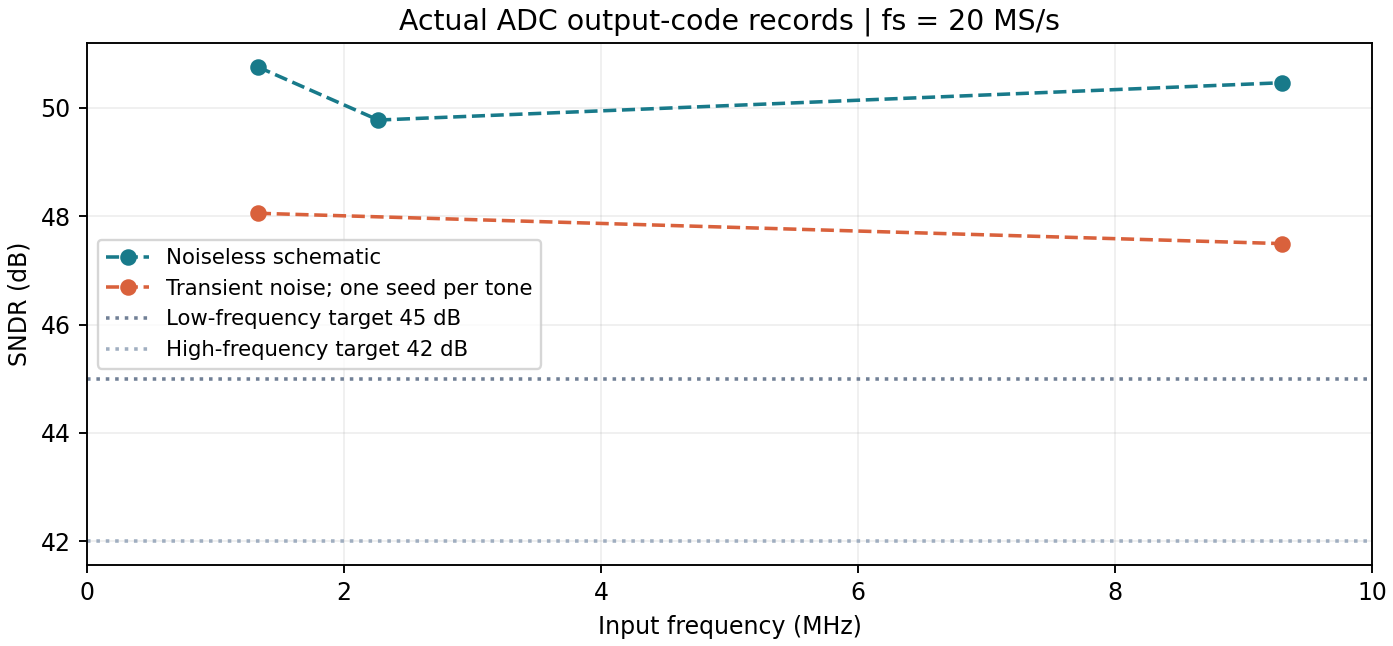
\includegraphics[width=\columnwidth]{../figures/sndr_vs_fin.png}
\caption{Historical output-code SNDR at the saved tones. The plotted values summarize the archived code records; no new analog simulation is introduced by this report.}\label{fig:sndr}
\end{figure}

\subsection{Static Linearity and History}
Noiseless TT, SS, FF, SF, and FS datasets contain 553 observations each and observe all 256 codes. All 255 transition brackets include an input guard. Endpoint fitting removes offset and gain; the fitted LSB uncertainty is propagated into the reported intervals. DNL covers interior codes 1--254 because the saturated end bins do not have two bounded transition edges. The worst retained magnitudes across the saved bounds are 0.251154\,LSB DNL and 0.190113\,LSB INL, inside the declared $\pm0.5$ and $\pm1$\,LSB limits.

The reverse-history equality diagnostic remains \emph{false}: 69 of 70 selected anchors agree. At exactly zero differential input, positive preceding history produces code 128 and negative preceding history produces 127. Under both tested relative tolerances, 0.001 and 0.0001, the selected $\pm20$\,$\mu$V probes produce the adjacent expected codes. This local observation does not eliminate history dependence at the transition.

The selected central-history band is approximately $[-21,+21]$\,$\mu$V after guards. The earlier forward bracket extends farther positive. The final $T_{128}$ interval therefore retains their union, approximately $[-21,+485.498]$\,$\mu$V; it is not narrowed to the newer band. Other transitions retain their original forward brackets. The saved reverse anchors do not verify every possible input history.

\subsection{Power and Export Boundaries}
AVDD power is a saved aggregate measured by the original testbench over adaptive internal timesteps. Ideal reference-high, reference-low, common-mode, and clock-source contributions are recorded separately with their signs. Negative contributions indicate returned energy. The published analysis checks aggregate arithmetic but does not reintegrate raw supply currents. Physical input, reference, and clock drivers are not implemented or included in a complete system-power budget.

Historical saved-and-reopened CAD export checks and an eight-conversion DC smoke test establish only their stated export scope. They do not replace dynamic or static ADC verification. The tighter central-boundary result was recovered from a complete saved transient and an error-free log after empty result files; its original process exit code remains unknown. Recovery-time model hashes cannot independently prove the earlier state of external model files.

\section{Reproduction and Remaining Work}
The repository's standard-library Python tools verify release hashes and recompute code spectra, deterministic bracket bounds, the central-history union, and the nominal hierarchy count. They retain the failed reverse diagnostic. These commands do not load a process model or run Spectre:
\begin{quote}\small\ttfamily
python tools/verify\_release.py\\
python tools/reproduce\_all.py --outdir reproduced
\end{quote}
The output directory must be new. The symbolic connectivity export contains undefined \texttt{NMOS\_CORE} and \texttt{PMOS\_CORE} names. A transistor rerun needs authorized compatible models, complete native instance parameters and options, and a reviewed external stimulus and measurement fixture. Substituting arbitrary generic models is not equivalent reproduction.

The schematic prototype has no qualified capacitor mismatch, extracted parasitics, layout area, DRC/LVS/PEX, voltage/temperature sweep, yield, extensive noisy-corner ensemble, or silicon result. The exact 3-dB effective-resolution bandwidth crossing is unmeasured. These limitations are unchanged by the new CircuitikZ presentation.

\section{Conclusion}
The saved experiments support an eight-bit, 20-MS/s schematic prototype with ideal capacitor arrays and 7.597--7.690 ENOB in two short transient-noise records. The publication preserves both bounded static linearity and the failed exact-zero reverse-history diagnostic. The editable drawings connect those results to the implemented CDAC switches, comparator storage, and native controller without extending the verification claims.

\begin{thebibliography}{1}
\bibitem{repo} SAR ADC Project, \emph{Authored Connectivity and Saved ADC Verification Exports}. [Online]. Available: \url{https://github.com/handsomegary/sar-adc-8bit}.
\end{thebibliography}
\end{document}
